\section{Função de Verossimilhança de Bernoulli}

\begin{frame}{O que é Verossimilhança?}
    \begin{itemize}
        \item Até o momento, avaliamos o ajuste de modelos por meio de critérios puramente geométricos (como a minimização do Erro Quadrático Médio).
        \item A \textbf{Função de Verossimilhança} ($L$) nos permite estimar parâmetros de modelos sob uma perspectiva probabilística.
        \item \textbf{Cenário Dedutivo (Probabilidade):}
        \begin{itemize}
            \item Os parâmetros populacionais $\theta$ são conhecidos (ex: moeda justa, $\theta = 0.5$).
            \item Queremos calcular a chance de observar um determinado conjunto de dados.
        \end{itemize}
        \item \textbf{Cenário Indutivo (Inferência/Verossimilhança):}
        \begin{itemize}
            \item Os dados amostrais já foram coletados e estão fixos.
            \item Queremos avaliar a plausibilidade de diferentes valores do parâmetro $\theta$.
        \end{itemize}
    \end{itemize}
\end{frame}

\begin{frame}{O Modelo Discreto: Ensaios de Bernoulli}
    \begin{itemize}
        \item Considere uma sequência de lançamentos de moedas independentes.
        \item Cada lançamento $X_i \in \{0, 1\}$ segue uma distribuição de Bernoulli com $P(X_i = 1) = \theta$.
        \item A Função de Massa de Probabilidade ($PMF$) de Bernoulli é escrita como:
        $$P(X_i = x_i) = \theta^{x_i} (1 - \theta)^{1 - x_i}$$
        \item Assumindo observações independentes e identicamente distribuídas, a \textbf{Função de Verossimilhança} de uma amostra de tamanho $N$ é o produto das PMFs individuais:
        $$L(\theta) = \prod_{i=1}^N P(X_i = x_i) = \prod_{i=1}^N \theta^{x_i} (1 - \theta)^{1 - x_i}$$
        $$L(\theta) = \theta^{\sum_{i=1}^N x_i} (1 - \theta)^{N - \sum_{i=1}^N x_i}$$
    \end{itemize}
\end{frame}

\begin{frame}{Visualizando a Verossimilhança de Bernoulli}
    \begin{columns}
        \begin{column}{0.5\textwidth}
            \textbf{Experimento Prático:}
            \begin{itemize}
                \item Jogamos uma moeda $N = 13$ vezes e observamos $4$ caras ($1$) e $9$ coroas ($0$).
                \item A função de verossimilhança é:
                $$L(\theta) = \theta^4 (1 - \theta)^9$$
                \item \textbf{Ponto de Máximo:}
                Graficamente, a plausibilidade é maximizada em $\theta \approx 0.3077$.
                \item \textbf{Desafio Numérico:}
                Os valores de $L(\theta)$ são muito pequenos (na ordem de $10^{-4}$).
            \end{itemize}
        \end{column}
        \begin{column}{0.5\textwidth}
            \centering
            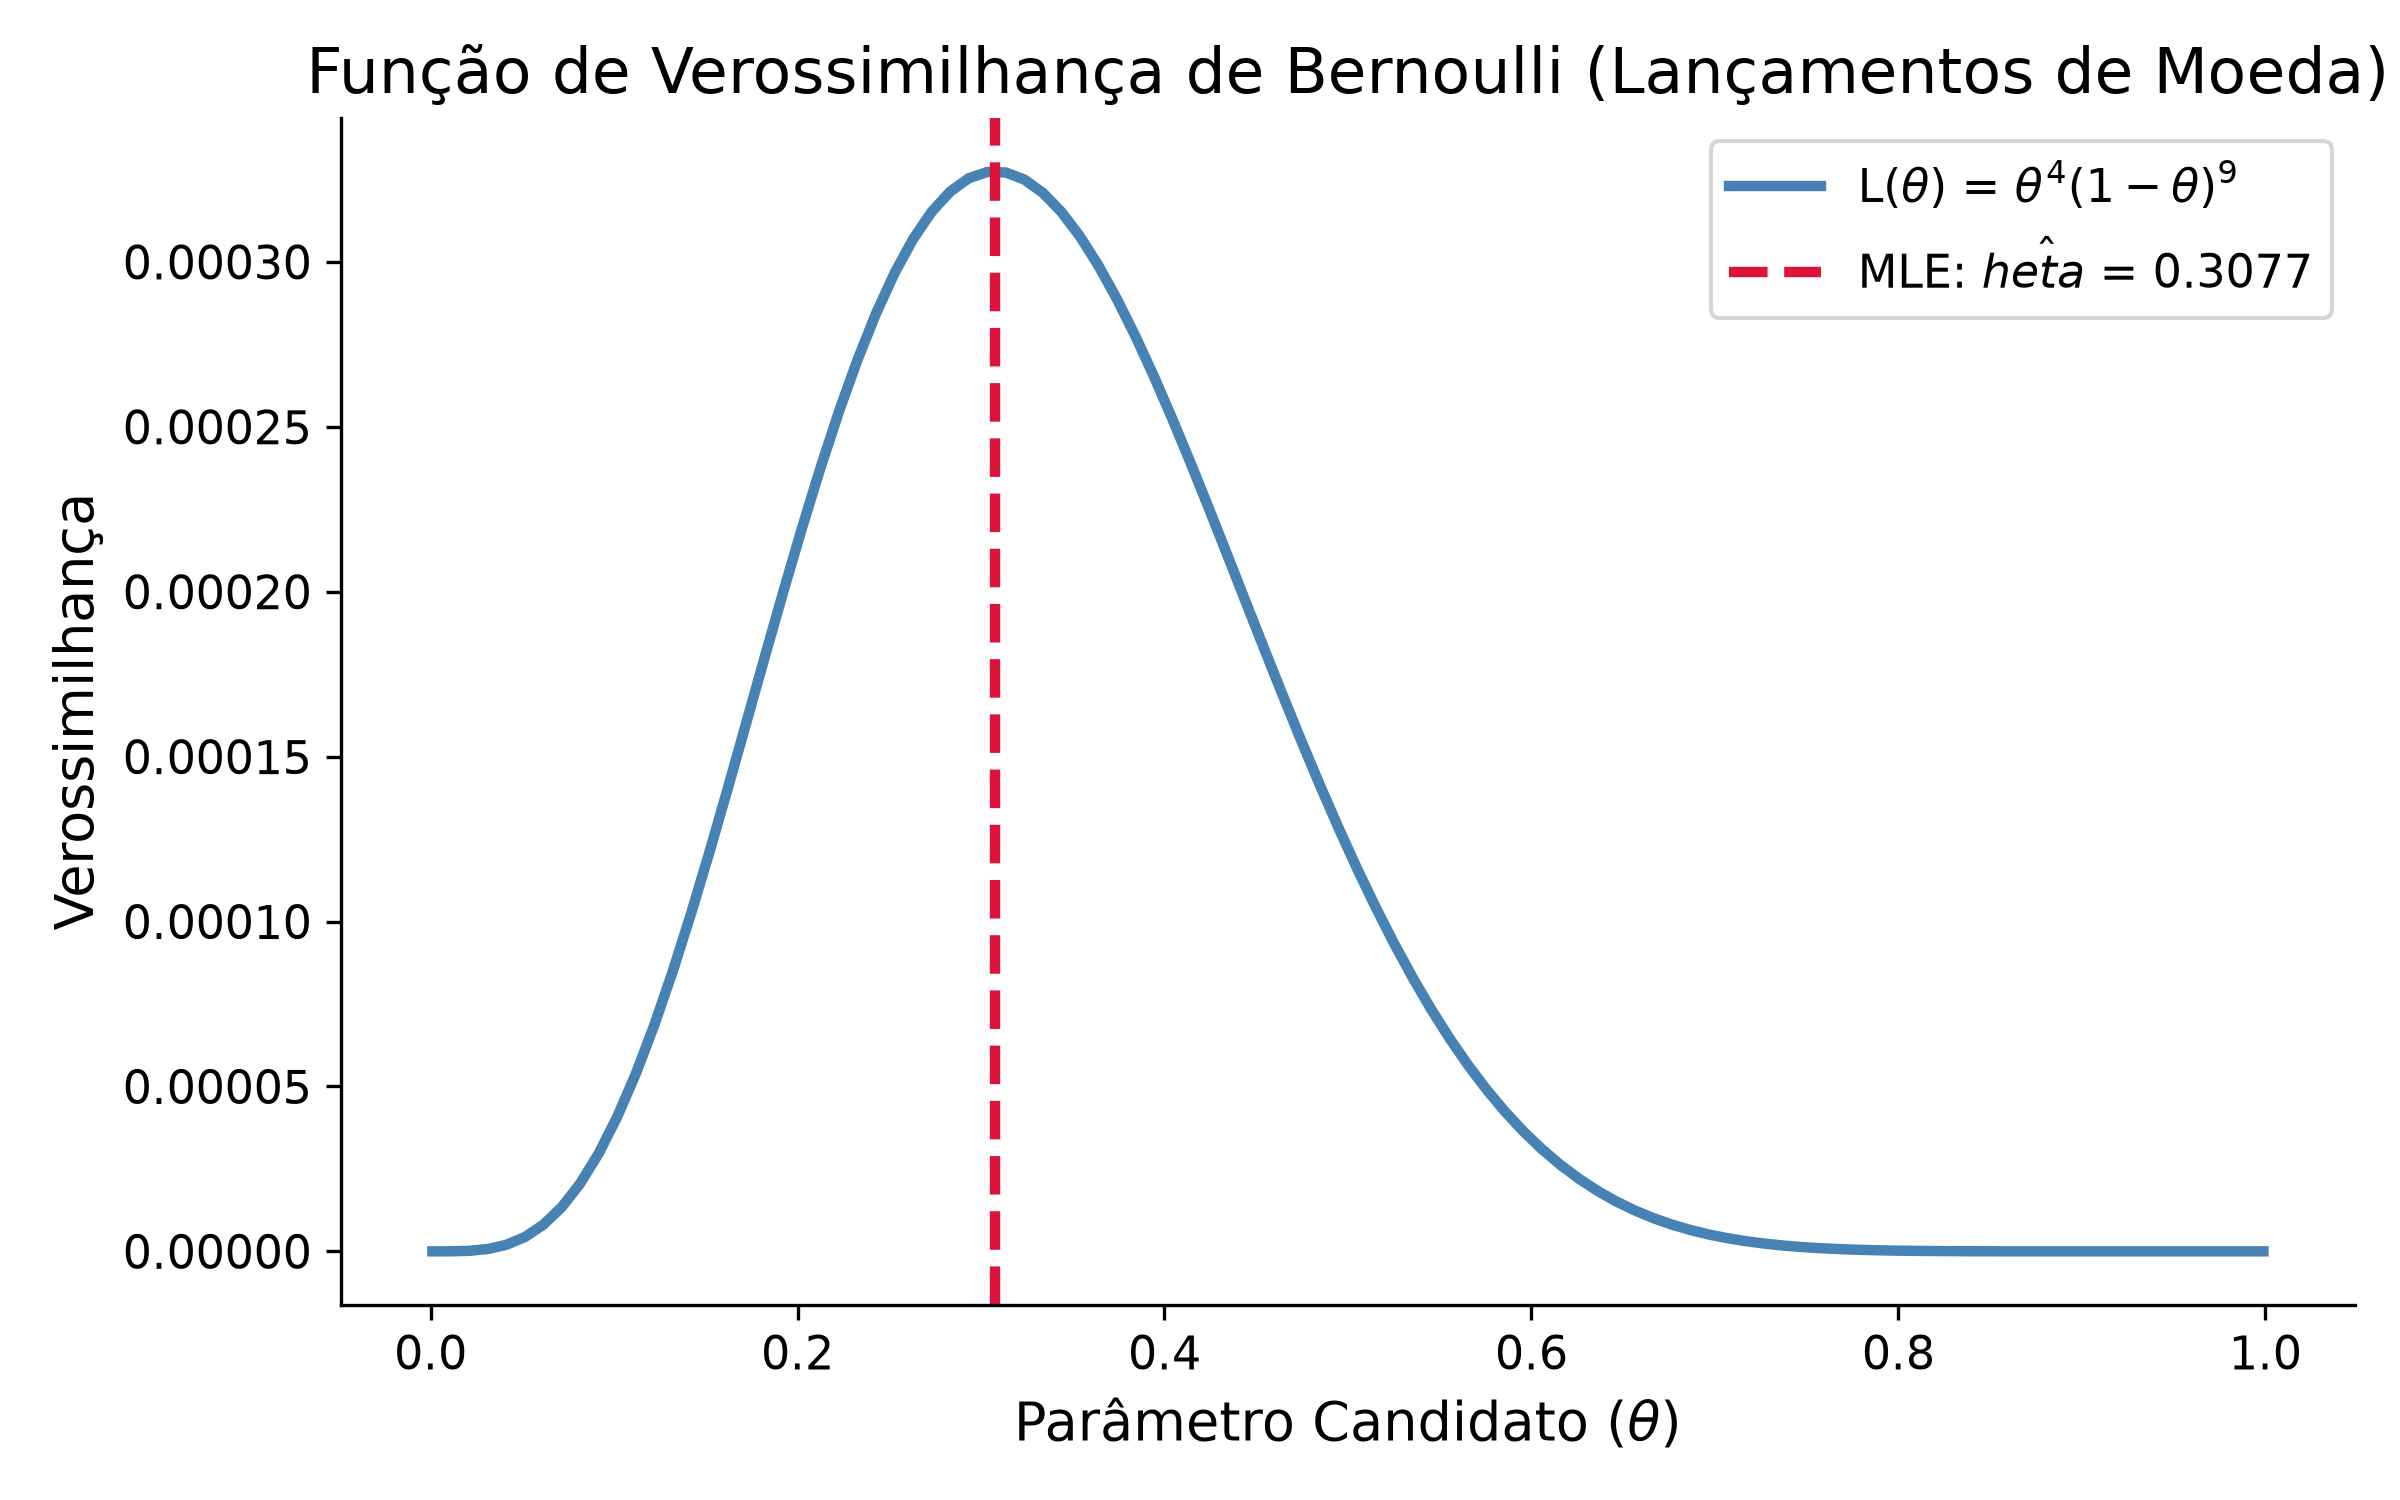
\includegraphics[width=\textwidth]{verossimilhanca_bernoulli.png}
        \end{column}
    \end{columns}
\end{frame}

\begin{frame}{A Escala de Log-Verossimilhança}
    \begin{itemize}
        \item Para computadores, multiplicar dezenas ou centenas de probabilidades menores que 1 gera \textbf{subfluxo numérico} (underflow), onde o produto é arredondado para zero.
        \item Aplicando a função de logaritmo natural ($\ln$) na verossimilhança, convertemos produtos em somatórios:
        $$\ln L(\theta) = \ln \left( \prod_{i=1}^N P(X_i = x_i) \right) = \sum_{i=1}^N \ln P(X_i = x_i)$$
        \item Como a função $\ln(y)$ é estritamente crescente, o valor de $\theta$ que maximiza a log-verossimilhança é o mesmo que maximiza a verossimilhança original.
        \item Para o caso de Bernoulli:
        $$\ln L(\theta) = \left( \sum_{i=1}^N x_i \right) \ln \theta + \left( N - \sum_{i=1}^N x_i \right) \ln(1 - \theta)$$
    \end{itemize}
\end{frame}

\begin{frame}{Visualizando a Log-Verossimilhança}
    \begin{columns}
        \begin{column}{0.5\textwidth}
            \textbf{Escala de Log-Verossimilhança:}
            \begin{itemize}
                \item O valor máximo da curva ocorre no mesmo ponto:
                $$\theta \approx 0.3077$$
                \item A escala no eixo vertical agora varia em valores negativos mais estáveis (não decai para zero).
                \item Facilita a modelagem computacional e a obtenção das derivadas.
            \end{itemize}
        \end{column}
        \begin{column}{0.5\textwidth}
            \centering
            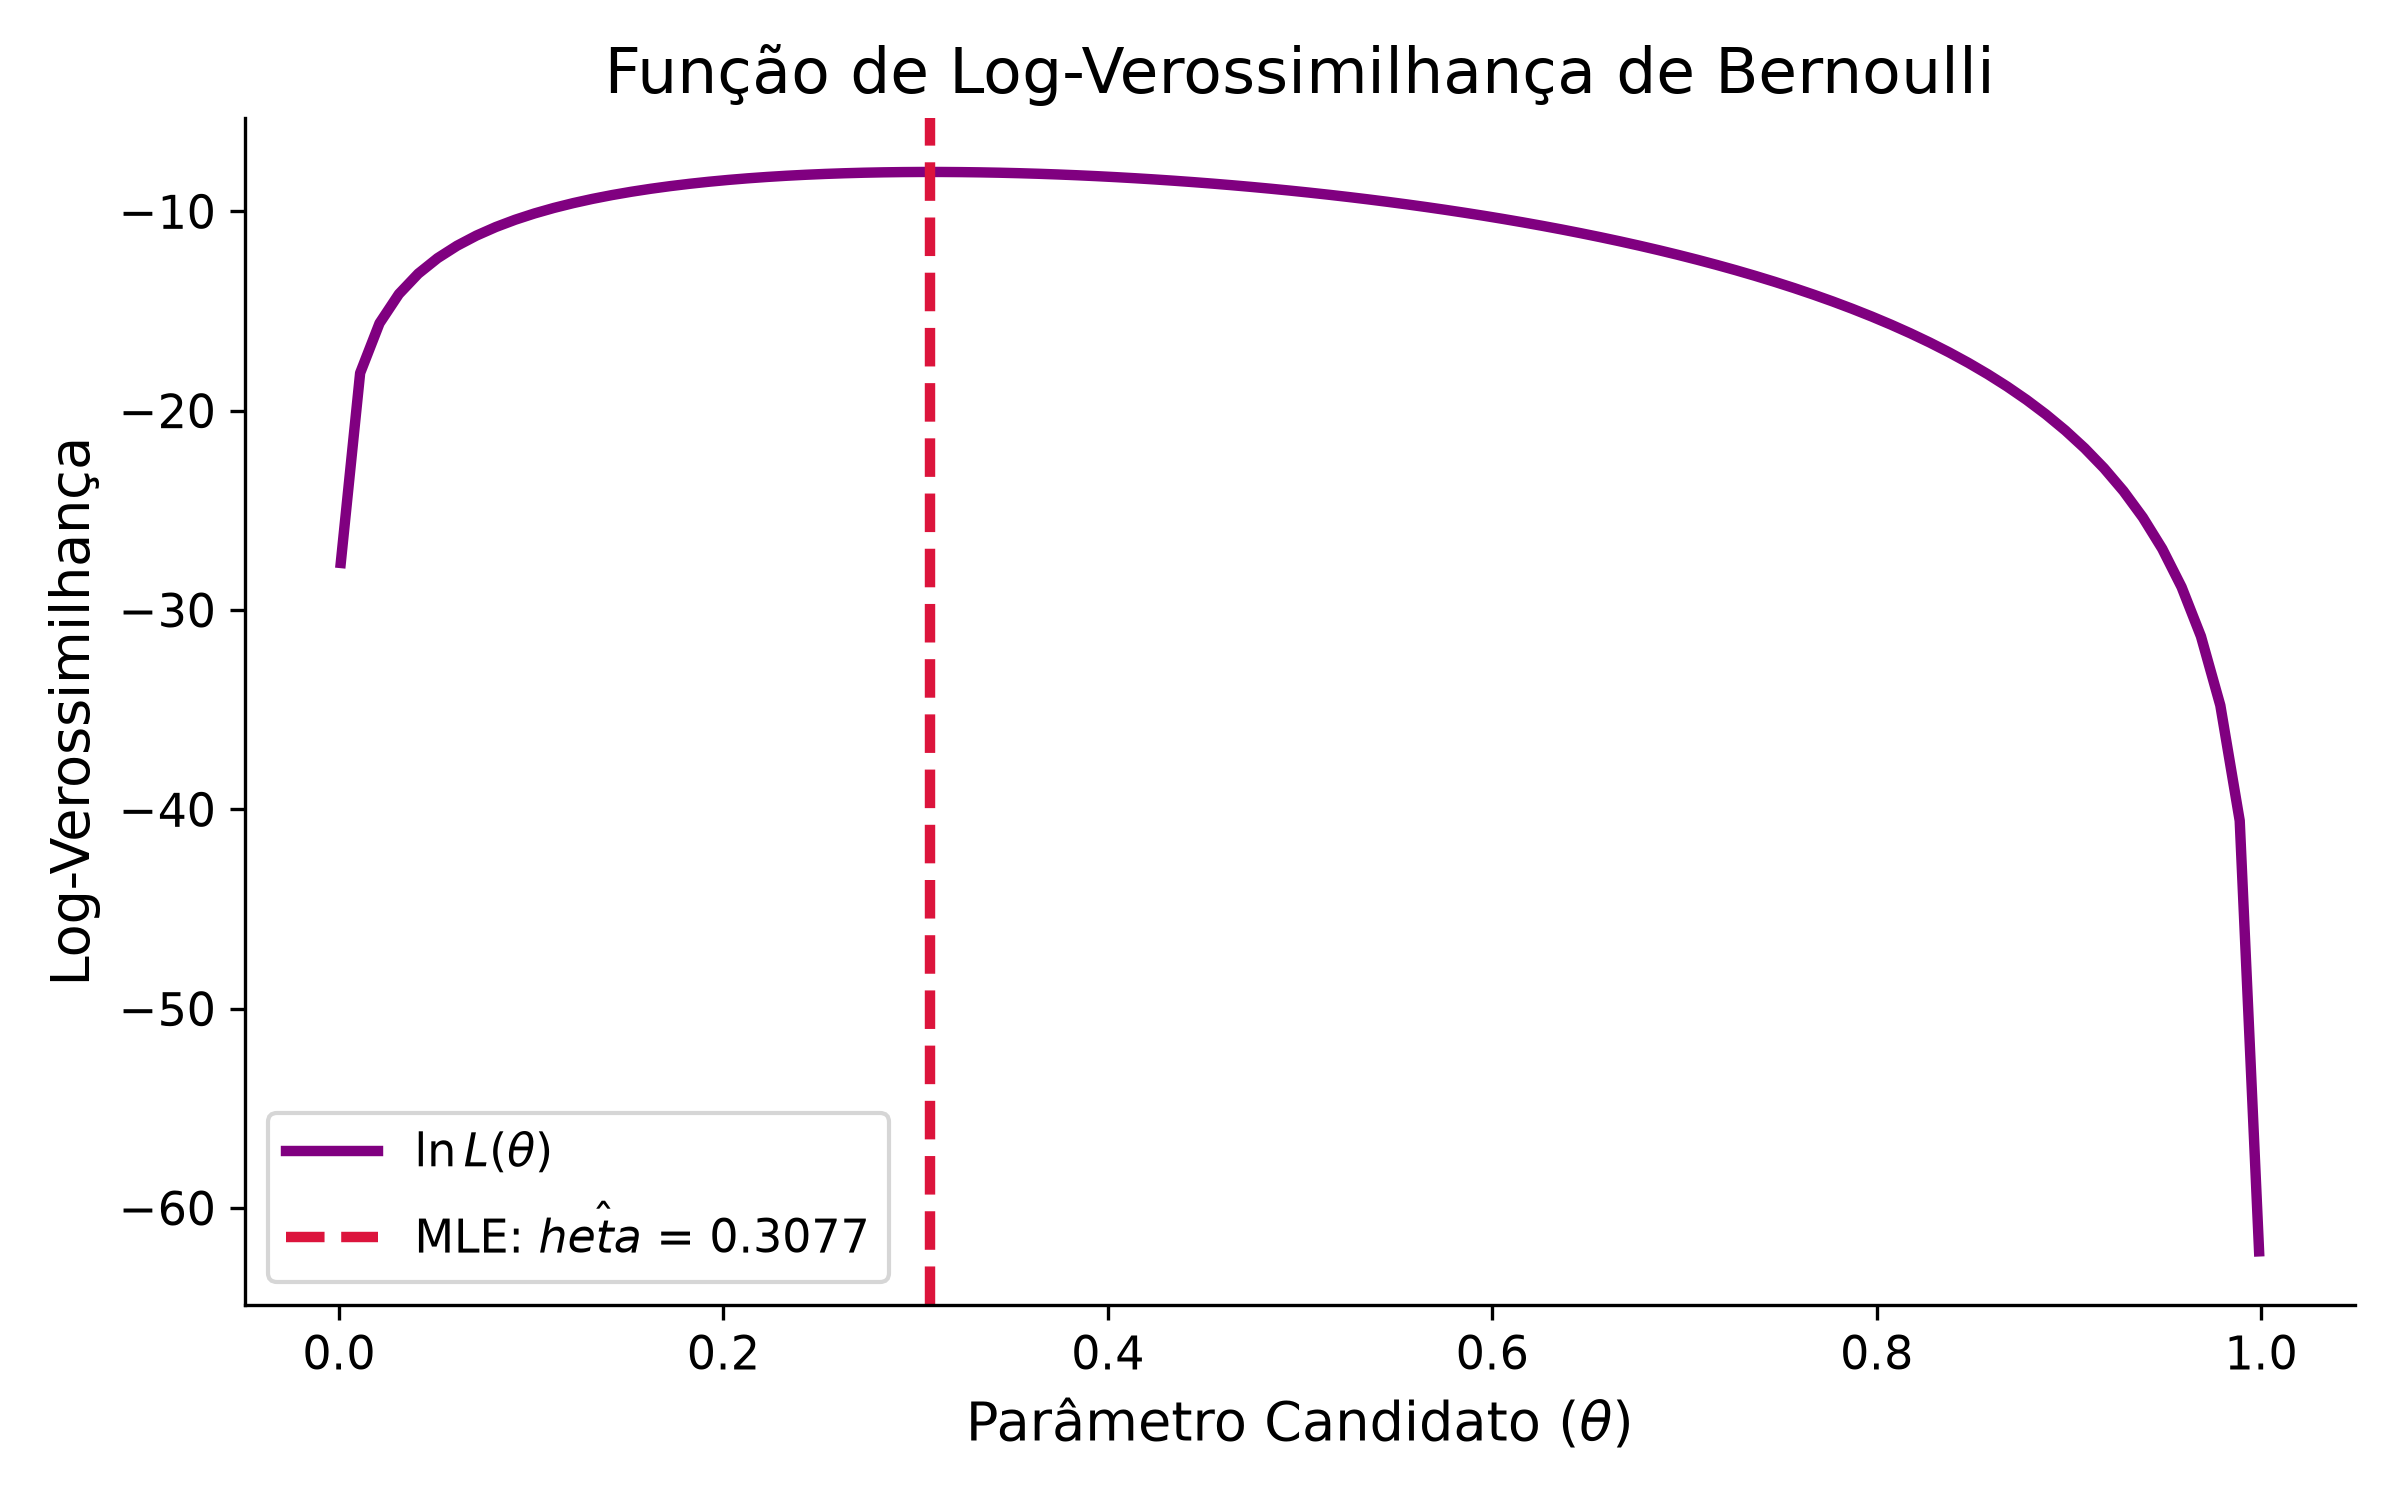
\includegraphics[width=\textwidth]{log_verossimilhanca_bernoulli.png}
        \end{column}
    \end{columns}
\end{frame}

\begin{frame}{Exemplo Pareado: Solução Analítica}
    \begin{itemize}
        \item Queremos encontrar o valor de $\theta$ que maximiza a log-verossimilhança:
        $$\ln L(\theta) = (\sum x_i) \ln \theta + (N - \sum x_i) \ln(1 - \theta)$$
        \item Derivamos com relação ao parâmetro $\theta$ e igualamos a zero para achar o ponto crítico:
        $$\frac{d \ln L(\theta)}{d\theta} = \frac{\sum x_i}{\theta} - \frac{N - \sum x_i}{1 - \theta} = 0$$
        $$\frac{\sum x_i}{\theta} = \frac{N - \sum x_i}{1 - \theta} \implies (1 - \theta) \sum x_i = \theta (N - \sum x_i)$$
        $$\sum x_i - \theta \sum x_i = \theta N - \theta \sum x_i \implies \hat{\theta}_{MLE} = \frac{\sum x_i}{N}$$
        \item \textbf{Conclusão:} A Estimativa de Máxima Verossimilhança ($\hat{\theta}_{MLE}$) para a proporção é a própria proporção amostral dos dados.
    \end{itemize}
\end{frame}

\begin{frame}[fragile]{Exemplo Pareado: Implementação em Python}
    \begin{block}{Calculando a Log-Verossimilhança de Bernoulli}
\begin{lstlisting}
import numpy as np

# Dados do experimento (4 caras, 9 coroas)
dados = np.array([1, 1, 1, 1, 0, 0, 0, 0, 0, 0, 0, 0, 0])
N = len(dados)
sucessos = np.sum(dados)
fracassos = N - sucessos

# Proporcao empirica (MLE)
theta_otimo = sucessos / N
print(f"MLE de theta: {theta_otimo:.4f}") # Saida: 0.3077

# Funcao de log-verossimilhanca
def log_verossimilhanca(theta, k, n):
    return k * np.log(theta) + (n - k) * np.log(1 - theta)

# Testando valores candidatos de theta
for theta in [0.1, 0.3077, 0.5, 0.8]:
    ll = log_verossimilhanca(theta, sucessos, N)
    print(f"Theta: {theta:.4f} | Log-Verossimilhanca: {ll:.4f}")
\end{lstlisting}
    \end{block}
\end{frame}
